\section{Introduction}

\def\Z{\mathbb{Z}}
\def\R{\mathbb{R}}
\begin{frame}
	\frametitle{Discrete Time Signal}
	\begin{definition}
		Discrete time signals are sequences of values at the moments \dots,-2T,-T,0,T,2T,\dots.\\
		$x[k]$ is the value of a signal at the moment $t = kT$
	\end{definition}
	\begin{example}
		\begin{figure}
			\centering
			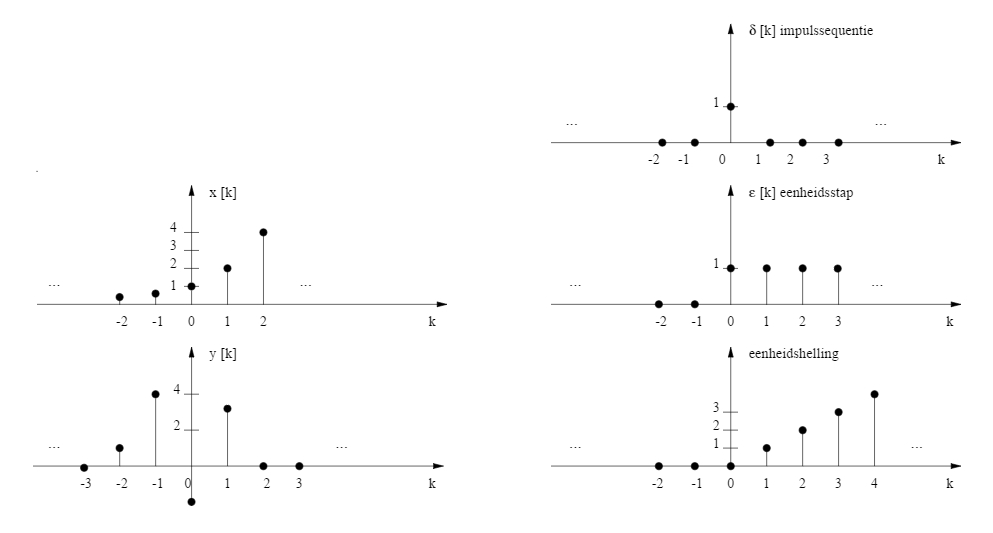
\includegraphics[height=0.4\textheight]{Images/discrete_time_systems_13}
			\caption{}
			\label{fig:discrete_time_systems_13}
		\end{figure}
	\end{example}
\end{frame}
\begin{frame}
	\frametitle{Discrete Time System}
	\begin{definition}
			A linear time-invariant (LTI) discrete time system processes an inputvector $u[k]$ to an outputvector $y[k]$.\\
			Such a system has:\\
			\begin{itemize}
				\item A vector of input $u[k]$
				\item A vector of output $y[k]$
				\item A vector of states $x[k]$
			\end{itemize}
	\end{definition}
\end{frame}
\begin{frame}
	\frametitle{Discrete Time System}
		\begin{example}
			\begin{figure}
			\centering
			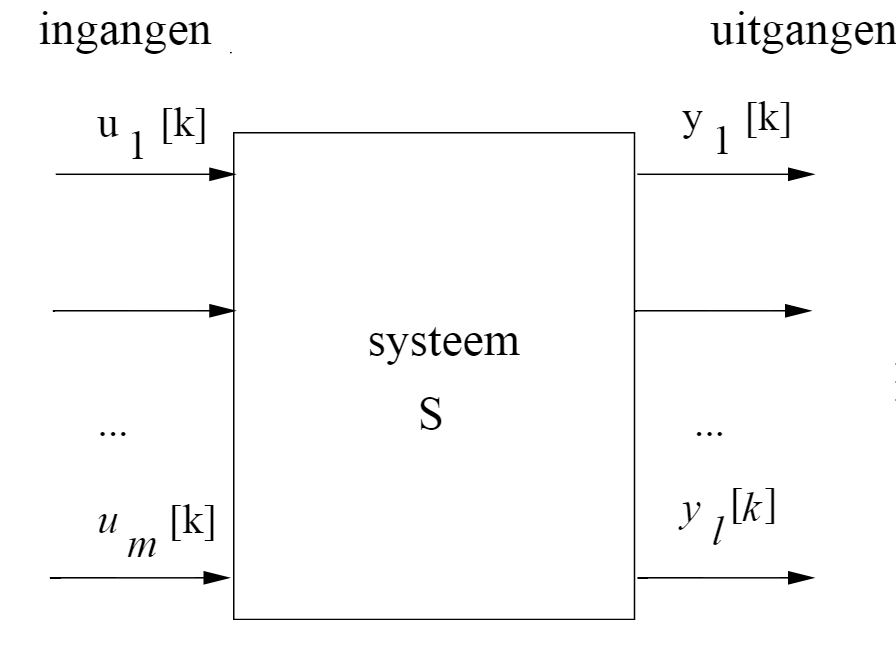
\includegraphics[height=0.7\textheight]{Images/discrete_time_systems_14}

			\label{fig:discrete_time_systems_14}
		\end{figure}

		\end{example}
\end{frame}
\begin{frame}
	\frametitle{How to represent a system?}
	\begin{itemize}
		\item Block-diagram
		\item State space representation
		\item Difference/differential equation
		\item Impulse response
		\item Transferfunctions
	\end{itemize}

\end{frame}
\section{Block-diagram}
\begin{frame}
	\frametitle{Block diagram}
	\begin{figure}
		\centering
		\label{fig:discrete_time_systems_2}
		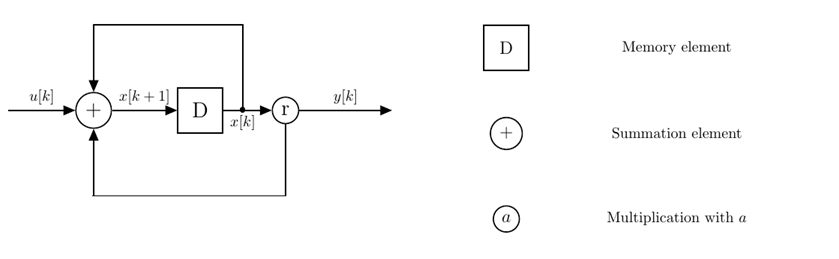
\includegraphics[width=0.75\linewidth]{Images/discrete_time_systems_2}
		\caption{An example of a discrete time system}
	\end{figure}
	\begin{definition}
			A block diagram is a visual representation of a system. All LTI’s (Linear Time Invariant) systems can be constructed using 3 building blocks(Memory element, summation element, multiplication element). Note that every memory element corresponds to one state variable.
	\end{definition}
\end{frame}
\begin{frame}
	\frametitle{Building blocks}
	\begin{columns}
		\begin{column}{0.33\textwidth}
			\begin{block}{Adder}
				\begin{figure}
				\centering
				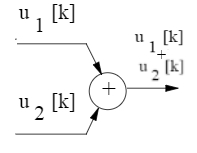
\includegraphics[width=0.7\linewidth]{Images/discrete_time_systems_15}
				\label{fig:discrete_time_systems_15}
			\end{figure}

			\end{block}
		\end{column}
		\begin{column}{0.33\textwidth}
				\begin{block}{Constant Multiplier}
					\begin{figure}
					\centering
					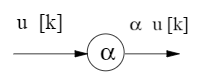
\includegraphics[width=0.7\linewidth]{Images/discrete_time_systems_16}
					\label{fig:discrete_time_systems_16}
					\end{figure}

				\end{block}
		\end{column}
		\begin{column}{0.33\textwidth}
			\begin{block}{Delay element}
				\begin{figure}
					\centering
					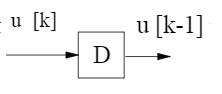
\includegraphics[width=0.7\linewidth]{Images/discrete_time_systems_17}
					\label{fig:discrete_time_systems_17}
				\end{figure}
			\end{block}
		\end{column}
	\end{columns}
\end{frame}
\begin{frame}
	\frametitle{Example: compond interes}
	\begin{itemize}
			\item $ u[k]$:The deposits and withdrawals from the bank account
			\item $ x[k]$:The current saldo on bank account(before deposit and interest)
			\item $ y[k]$: The acquired interest of that year
			\item $ x[k+1]$: The saldo on the next year = current saldo + interest + deposits
	\end{itemize}

	\begin{figure}
		\centering
		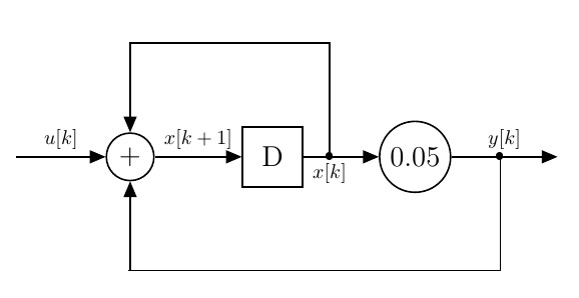
\includegraphics[height=0.45\textheight]{Images/discrete_time_systems_3}
		\label{fig:discrete_time_systems_3}
	\end{figure}
\end{frame}
\begin{frame}
	\begin{tabular}{|c|c|c|c|}
		\hline  $u[k]$& $x[k+1]$  & $x[k]$  & $y[k]$  \\ 
		\hline  50 & 50 & 0  & 0  \\ 
		\hline  0 & 52.5  & 50 & 2.5  \\ 
		\hline  -25 & 30.13 & 52.5 & 2.62  \\ 
		\hline  0 &  31.63 & 30.13  & 1.51  \\ 
		\hline  0 & 33.21  & 31.63 & 1.58 \\ 
		\hline  30 & 64.87 & 33.21  & 1.66 \\ 
		\hline  0 & 68.12 & 64.87 & 3.24  \\ 
		\hline  0 & 71.52 & 68.12 & 3.41 \\
		\hline 
	\end{tabular}
	

\end{frame}
\begin{frame}
	\frametitle{Bad block diagrams}

				\begin{alertblock}{Delay-free loops}
					The issue is that this leads to an implicit connection 
					$u[k]$ depends on $y[k]$ ,which is not yet known
					You can easily rewrite this in an allowd shape
					$y[k] = u[k]  + 3 y[k] \Longleftrightarrow y[k] = -\frac{1}{2} u[k]$
					\begin{figure}
						\centering
						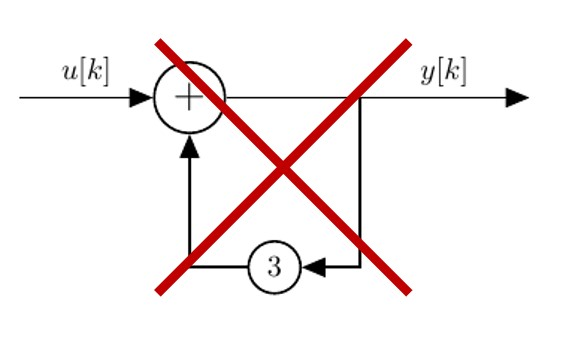
\includegraphics[width = 0.5\linewidth]{Images/discrete_time_systems_4}
						\caption{An example of a delay free loop}
						\label{fig:discrete_time_systems_4}
					\end{figure}
				\end{alertblock}

		

				

\end{frame}
\begin{frame}
	\frametitle{Bad block diagrams}
		\begin{alertblock}{Connecting two outputs without using a sum}
			The issue is that this can lead to inconsistencies.	According to this block diagram the output of the systems S1 and S2 are equal.There is no way to get around this.
			\begin{figure}
				\centering
				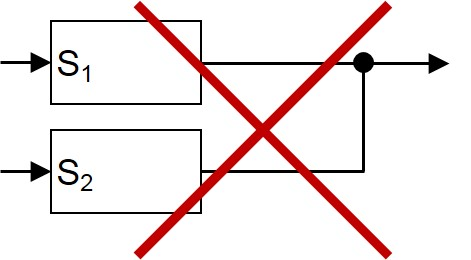
\includegraphics[width = 0.5\linewidth]{Images/discrete_time_systems_5}
				\label{fig:discrete_time_systems_5}
			\end{figure}
		\end{alertblock}
\end{frame}
\section{State Space representation}
\begin{frame}
	\frametitle{State space representation}
	\begin{definition}{State space representation}
		\begin{center}
			$x[k+1] = A x[k] + B u[k]$ \\
			$y[k] = C x[k] + D u[k] $ \\
		\end{center}
	\end{definition}
	This state space representation is specific to LTI systems:\\
	Linear: it’s easy to see these systems are linear \\
	Time-invariant: the matrices A,B,C,D do not depend on time, if it were to be a time-variant system the matrices would be replaced by $A[k], B[k], C[k] and D[k]$. \\
\end{frame}
\begin{frame}
\frametitle{From block diagram to state space }
\begin{columns}

\begin{column}{0.5\textwidth}
	\begin{block}{Blockdiagram}
		\begin{figure}
			\centering
			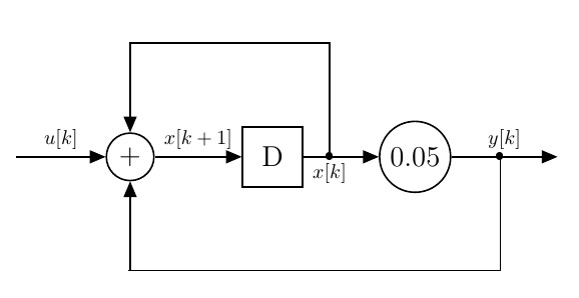
\includegraphics[width=1\linewidth]{Images/discrete_time_systems_3}
			\label{fig:discrete_time_systems_3}
		\end{figure}
	\end{block}
	
\end{column}
\begin{column}{0.5\textwidth}
	\begin{block}{State space representation}
		\begin{enumerate}
			\item Let the output of the memory elements be $x_{i}[k]$. 
			\item So the input of the memory elements are $x_{k+1}$
			\item Trace back to retrieve equations for $x_i[k+1] $   and $y_i[k]$ 
		\end{enumerate}
		This results in:
		\begin{center}
				$x[k+1] = u[k] + 1.05 x[k] $
				$y[k] = 0.05 x[k]$
		\end{center}
	\end{block}
\end{column}
\end{columns}
\end{frame}
\begin{frame}
	\frametitle{From state space to block diagram }
		\begin{block}{State space representation}
				\begin{center}
					$x[k+1] = A x[k] + B u[k]$ \\
					$y[k] = C x[k] + D u[k] $ \\
					
					with  A = 
					$\begin{bmatrix}
					1 & 0 & 0 \\
					0 & 0 & 1 \\
					0 & 3 & 0
					\end{bmatrix}$,
					B = 
					$\begin{bmatrix}
					1\\
					0\\
					4\\
					\end{bmatrix}$,
					C = 
					$\begin{bmatrix}
					5 & 1 & 0
					\end{bmatrix}$ 
					and D = 
					$\begin{bmatrix}
					1
					\end{bmatrix}$ \\
				\end{center}
		\end{block}
	\begin{block}{Blockdiagram}
		\begin{enumerate}
			\item First add a delay element for every state $x_i[k]$
			\item 	Determine the input for every state x[k+1] from the matrixes A and B, as a combination of the states x[k] and inputs u[k]
			\item Determine the outputs y[k] in the same way with the matrixes C and D
		\end{enumerate}
	
	\end{block}
	


\end{frame}
\begin{frame}
	\frametitle{From state space to block diagram (DT)}
	\begin{figure}
		\centering
		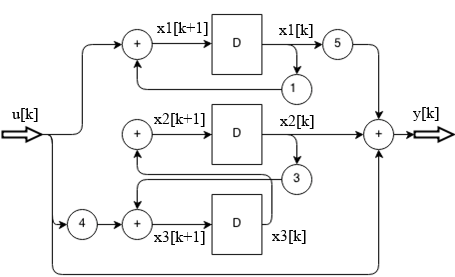
\includegraphics[width=0.7\linewidth]{Images/discrete_time_systems_18}
		\caption{}
		\label{fig:discrete_time_systems_18}
	\end{figure}

	
\end{frame}
\begin{frame}
	\frametitle{Different state space representations}
	\begin{alertblock}{State space representation is not unique}
		Take the following system, which connects u[k] to y[k]:
		\begin{center}
			$x[k+1] = A x[k] + B u[k]$ \\
			$y[k] = C x[k] + D u[k] $ 
		\end{center}
		Now take a non-singular square matrix T and the following system. The relation between u[k] and y[k] will be the same.	
		\begin{center}
			$Tx[k+1] = TAT^{-1}Tx[k] + TBu[k]$\\
			$y[k] = C T^{-1}Tx[k] + Du[k]$
		\end{center}
		With $x' = Tx, A' = TAT^{-1},B' = TB,C' = CT^{-1}$ and $D'=D$,  we have found a different state space representation for this system.
		
	\end{alertblock}
\end{frame}
\begin{frame}
	\begin{block}{Solving state space equation}
			\begin{center}
				$x[k+1] = A x[k] + B u[k]$ \\
				$y[k] = C x[k] + D u[k] $ 
			\end{center}
			\vspace{-1em}
			We express $X[1],x[2],\dots$ in function of $x[0]$:
			\vspace{-1em}
			\begin{equation}
				\begin{align}
				$x[1] &= Ax[0]+Bu[0]$\\
				$x[2] &= Ax[1] + Bu[1] = A^2x[0]+ABu[0]+ Bu[1]$\\
				&\vdots\\
				$x[k] &= A^kx[0] + \sum\limits_{i=0}^{k-1} A^{k-1-i}Bu[i]$
				\end{align}
			\end{equation}
			\vspace{-1em}
			The output is $y[k]$:
			\begin{center}
				$y[k] = \left\{ \begin{matrix} Cx[0] + Du[0]  & \mbox{if k = 0} \\ CA^kx[0]+\sum\limits_{i=0}^{k-1} CA^{k  -1  -i}Bu[i] +D u[k] & \mbox{if k $> $0} \end{matrix}\right$
			\end{center}
	\end{block}
\end{frame}
\section{Diffence equations}
\begin{frame}
	\frametitle{Diffence equations}
	\begin{definition}
		Similar to differential equations, but for discrete time.\\
		General form: $\sum\limits_{i=0}^n a_iy[k+i] = \sum\limits_{i=0}^n b_iu[k+i]$\\
		With n  the order of the system.\\
	\end{definition}
	\begin{block}{Solution in 2 parts}
	\begin{enumerate}
			\item Homogenous: solution from input zero
			\item Particular: solution derived as a response from the input
	\end{enumerate}
	\end{block}
\end{frame}
\begin{frame}
	\frametitle{Homogenous difference equations}
	\begin{definition}
		General form: $\sum\limits_{i=0}^n a_iy[k+i]= 0$ \\
	\end{definition}
	\begin{example}
		$y[k+1] - ay[k] = 0$\\
		$y[k+1] = ay[k] $\\
		$y[1] = ay[0] $\\
		$y[2] = ay[1] = a^2y[0]$\\
		\vdots
		$y[n] = a^{n}y[0]$
	\end{example}

\end{frame}
\begin{frame}
	\frametitle{Homogenous difference equations}
	\begin{block}{solution}
		\begin{itemize}
			\item Expected form of solution: $r^{k}$ 
			\item 	Substitution of the expected solution in the difference equation:
			$\sum\limits_{i=0}^n a_ir^{k+i}= 0$
			\item Division by $r^{k}$ leads to the characteristic equation:
			$\sum\limits_{i=0}^n a_ir^{i}= 0$
			\item 	Solutions of the characteristic equation:
			$r_1,r_2,r_3,\dots$
			\item Homogenous solution to the difference equation: 
			$y[k] = c_1r_1^{k} + c_2r_2^{k} + c_3r_3^{k} + \cdots =\sum\limits_{i=1}^{n}c_ir_i^{k}$
		\end{itemize}
	\end{block}
\end{frame}
\begin{frame}
	\begin{example}
		
		\begin{itemize}
			\item Homogeneous recurrence relations: $y[k+2]-5y[k+1]+6y[k] = 0$
			\item Initial value: $y[0] =1$, $y[1] = 1$
			\item Characteristic polynomial: $r^2-5r+6=0$
			\item Roots: 2 and 3
			\item General solution: $c_1 2^k + c_2 3^k$
			\item Intital values: 
			\begin{center}
				$
				\begin{Bmatrix}
					1 = c_1 + c_2\\
					1 = 2c_1 + 3c_2\\
				\end{Bmatrix}
				$\\
					$
					\begin{Bmatrix}
					2 = c_1 \\
					-1 = c_2\\
					\end{Bmatrix}
					$\\
			\end{center}
			\item Result: $y[k] = 2^{k+1} - 3^{k}$
		\end{itemize}
	\end{example}
\end{frame}
\begin{frame}
\frametitle{Example: Fibonacci sequence}
\begin{columns}
	\begin{column}{0.35\linewidth}
		
\begin{figure}
\centering
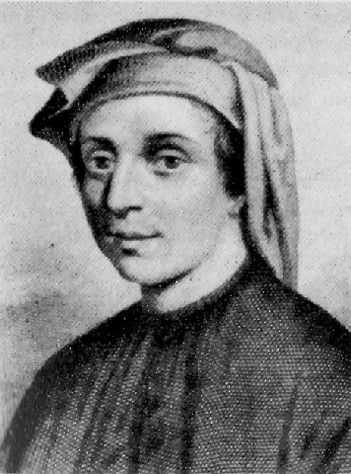
\includegraphics[height=0.5\textheight]{Images/discrete_time_systems_7}
\caption{\scriptsize{Leonardo Bonacci (c. 1170 – c. 1250)known as Fibonacci was an Italian mathematician, considered to be "the most talented Western mathematician of the Middle Ages".}}
\label{fig:discrete_time_systems_7}
\end{figure}
	\end{column}
	\begin{column}{0.65\linewidth}
\begin{figure}
\centering
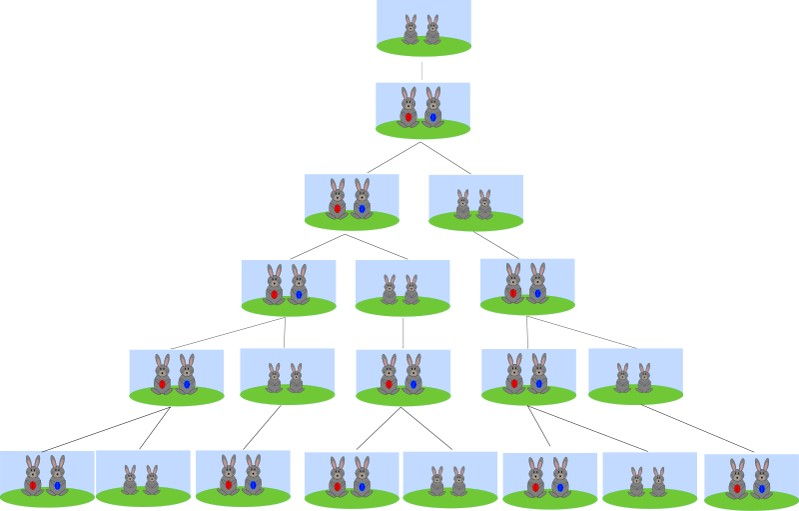
\includegraphics[width=0.9\linewidth]{Images/discrete_time_systems_8}
\caption{Fibonacci sequence}
\label{fig:discrete_time_systems_8}
\end{figure}
	\end{column}
\end{columns}
\end{frame}
\begin{frame}
	\frametitle{Example: Fibonacci sequence}
	\begin{example}
		\begin{itemize}
			\setlength\itemsep{0em}
			\item Homogeneous recurrence relations: $y[k+2] = y[k+1] + y[k]$
			\item Initial value: $y[0]=1, y[1]= 1$
			\item Characteristic polynomial: $r^2 - r - 1=0$ 
			\item Roots: $\frac{1+\sqrt{5}}{2}, \frac{1-\sqrt{5}}{2}$
			\item General solution: $y[k] = c_1(\frac{1+\sqrt{5}}{2}) + c_2(\frac{1-\sqrt{5}}{2})$
			\item Intital values: 
			\begin{center}
				$
				\begin{Bmatrix}
				c_1+ c_2 = 1\\
				c_1 \frac{1+\sqrt{5}}{2} + c_2 \frac{1-\sqrt{5}}{2} = 1  \\
				\end{Bmatrix}
				$\\
				$
				\begin{Bmatrix}
				c_1 = \frac{5+\sqrt{5}}{10}  \\
				c_2 = \frac{5-\sqrt{5}}{10}
				\end{Bmatrix}
				$\\
			\end{center}
			\item Result: $y[k] =  (\frac{5+\sqrt{5}}{10})(\frac{1+\sqrt{5}}{2}) +(\frac{5-\sqrt{5}}{10}) (\frac{1-\sqrt{5}}{2})$
		\end{itemize}
	\end{example}
\end{frame}
\begin{frame}
	\frametitle{Multiple roots and Complex roots}
	\begin{block}{Multiple roots}
		For a multiple root $r_i$ with multiplicity m add $r_i^k$,$kr_i^k$,\dots,$k^{m-1}r_i^{k}$
	\end{block}
	\begin{block}{Complex roots}
		\small{
		Complex  will result in oscillating behavior.
		If the difference equations and starting conditions are both real the complex roots can only be present in conjugate pairs, the constants will also be in conjugate pairs.
		\vspace{-1em}
		\begin{center}
				$ r_i = Re^{j\phi}$ 	$r_{i+1} = Re^{-j\phi}$\\
				$c_i = R_0e^{j\phi_0}$	 $c_{i+1} = R_0e^{-j\phi_0}$\\
				$c_ir_i^k+c_{i+1}r_{i+1}^k = R_0Re^{jk\phi+j\phi_0} +  R_0Re^{-(jk\phi+j\phi_0)} $\\
				This can be converted into a cosine using Euler’s formula:
				\vspace{-1em}
				\begin{multline*}
						y[k] = R_0R\big(\cos(k\phi+\phi_0) + \sin(k\phi+\phi_0) \big) +\\ R_0R\big(\cos(k\phi+\phi_0) - \sin(k\phi+\phi_0) \big)  
				\end{multline*}\\
						 $= 2R_0R\big(\cos(k\phi+\phi_0)\big)$			
		\end{center}}
	\end{block}
\end{frame}
\begin{frame}
	\frametitle{Euler’s formula}
	\begin{theorem}
		$e^{j\phi} = \cos(\phi) + \sin(\phi)j$
	\end{theorem}
	\begin{proof}
		Using power series:
			\begin{align*}
					$e^{\phi j} &= 1 + jx-\frac{x^{2}}{2!} - \frac{jx^{3}}{3!} + \frac{x^{4}}{4!} + \frac{jx^{5}}{5!} + \dots$\\
					& = \bigg(1-\frac{x^{2}}{2!}+ \frac{x^{4}}{4!} + \dots\bigg)+\bigg(x - \frac{x^{3}}{3!} + \frac{x^{5}}{5!}+\dots\bigg)j\\
					&= \cos(\phi) + \sin(\phi)j
			\end{align*}		
	\end{proof}
\end{frame}
\begin{frame}
	\frametitle{Non-homogeneous difference equations}
	\begin{definition}
		\begin{center}
			$\sum\limits_{i=0}^n a_iy[k+i] = \sum\limits_{i=0}^n b_iu[k+i]$\\
		\end{center}
	 	A linear combination of inputs results in the same linear combination of the outputs resulting from each input individually.
	\end{definition}
	\begin{block}{Solution}
		The equation can thus be solved for each input individually and the results added together afterwards.
			
		The resulting particular solutions can then be added to the general form of the homogenous solution.
	\end{block}
\end{frame}
\begin{frame}
	\frametitle{Particular solutions to difference equations}
	\begin{tabular}{|c|c|}
		\hline Input $u[k]$ & Suggested solution $y[k]$  \\ 
		\hline $k$ & $\alpha_1k+\alpha_0 $\\ 
		\hline $k^{n}$ & $\sum\limits_{i=0}^{n}\alpha_{i}k^{i}$ \\ 
		\hline $a^{k}$&  $\alpha a^{k}$\\ 
		\hline $k^{n}a^{k}$ & $(\sum\limits_{i=0}^{n}\alpha_{i}k^{i})a^{k}$  \\ 
		\hline $cos(k\phi)$ & $\alpha cos(k\phi + \phi_0)$\\ 
		\hline $a^{k}cos(k\phi)$ & $\alpha a^{k} cos(k\phi + \phi_0)$  \\ 
		\hline  $k^{n}a^{k}cos(k\phi)$&  $(\sum\limits_{i=0}^{n}\alpha_{i}k^{i}\alpha a^{k} cos(k\phi + \phi_0)$ \\ 
		\hline 
	\end{tabular} 
\end{frame}
\begin{frame}
	\frametitle{Example}
	\begin{example}
		\begin{itemize}
			\setlength\itemsep{0em}
			\item Difference equation : $y[k+2] - 5y[k+1]+6y[k]=(-1)^k$
			\item Initial value:  $y[1] = \frac{1}{4}, y[0] = \frac{1}{12}$
			\item Homogeneous difference equation: $y[k+2] - 5y[k+1]+6y[k] = 0$
			\item Characteristic polynomial: $r^2-5r+6 = 0$
			\item Homogeneous solution: $y_{hom}[k] = c_{1}2^{k} + c_{2}3^{k}$
			\item Particular solution: $y_{par}[k] = \alpha(-1)^k$
			\item Subsitution: $\alpha(-1)^{k+2}-5\alpha(-1)^{k+1}+6\alpha(-1)^k = (-1)^k$
			\item $\alpha = \frac{1}{12}$
			\item General solution: $y[k] = c_{1}2^{k}+c_{2}3^{k}+\frac{1}{12}(-1)^{k}$
			\item Initial values: $c_1 = -\frac{1}{3}, c_{2} = \frac{1}{3}$
			\item Result:  $y[k]= -\frac{1}{3}2^{k}+\frac{1}{3}3^{k}+\frac{1}{12}(-1)^{k}$
		\end{itemize}
	\end{example}

\end{frame}
\section{Impulse response and convolution}
\begin{frame}
	\frametitle{Impulse responses }
	\begin{definition}
			$\delta[k] = \left\{ \begin{matrix} 1  & \mbox{if k = 0} \\ 0 & \mbox{otherwise } \end{matrix}\right$
	\end{definition}
	\begin{figure}
\centering
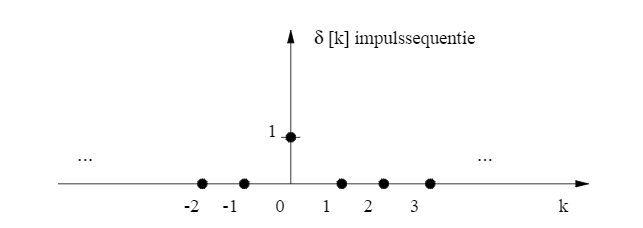
\includegraphics[width=0.6\linewidth]{Images/discrete_time_systems_19}
\label{fig:discrete_time_systems_19}
\end{figure}
\begin{theorem}
	You can decompose any signal in a sum of impulse response:s\\
	$f[k]=\sum\limits_{i=-\infty}^{i=\infty}\delta[k-i]f[i] = \delta[k] \ast f[k]$
\end{theorem}
\end{frame}
\begin{frame}
	\frametitle{Convolution}
	\begin{definition}
		$w[k]=u[k]\ast v[k] = \sum\limits_{i=-\infty}^{\infty} u[i]v[k-i]$
	\end{definition}
	\begin{block}{Solve}
		\begin{enumerate}
			\item Flip v[i] around vertical axis(v[-i]).
			\item Slide to the right over k steps(v[k-i]).
			\item Multiply $u[i]$ and $v[k-i]$
			\item Sum all the vaules.
		\end{enumerate}
	\end{block}
\end{frame}
\begin{frame}
	\frametitle{Convolution theorem (DT)}
	\begin{theorem}
		$y[k] = u[k] \ast h[k]$
	\end{theorem}
	\begin{proof}
		\begin{center}
				$ \delta[k] \rightarrow h[k]$\\
				$ \delta[k+i] \rightarrow h[k+i]$\\
				$ \sum\limits_{i=-\infty}^{i=\infty}\delta[k-i]u[i] \rightarrow \sum\limits_{i=-\infty}^{i=\infty}h[k-i]u[i]$\\
				$u[k] \rightarrow u[k] \ast h[k] = y[k] $
		\end{center}
	\end{proof}
\end{frame}
\begin{frame}
	\begin{figure}
\centering
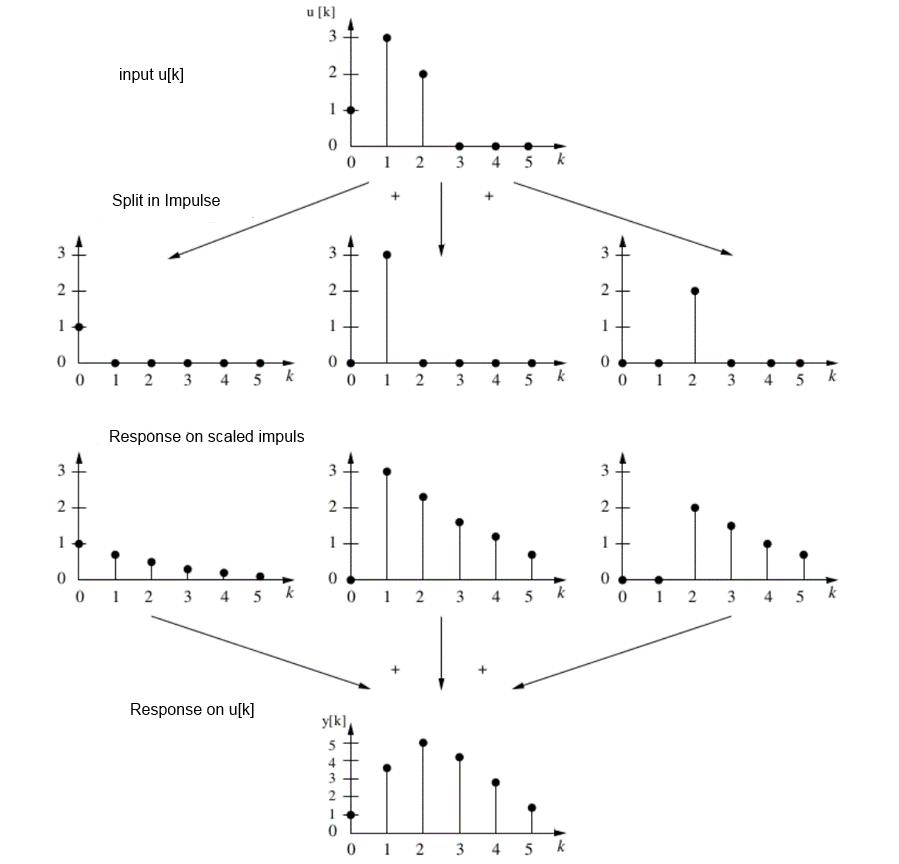
\includegraphics[width=0.7\linewidth]{Images/discrete_time_systems_20}
\caption{}
\label{fig:discrete_time_systems_20}
\end{figure}

\end{frame}
\begin{frame}
	\frametitle{Impulse response}
	\begin{definition}
		The impulse response of a dynamic system is its output when presented with a brief input signal, called an impulse.
	\end{definition}
	\begin{block}{Impulse response}
		$h[k] = \left\{ \begin{matrix} 0  & \mbox{if k$ <$  0} \\ D & \mbox{k= 0 }\\ CA^{k-1}B & \mbox{k$>$ 0 } \end{matrix}\right$
	\end{block}
\end{frame}
\begin{frame}
	\frametitle{Examples of Dirac-delta’s}
	Popping balloons for acoustic measurements
\begin{figure}
\centering
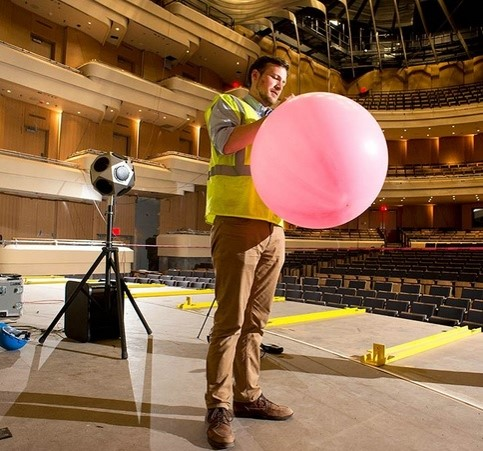
\includegraphics[height=0.7\textheight]{Images/discrete_time_systems_9}
\label{fig:discrete_time_systems_9}
\end{figure}

\end{frame}
\begin{frame}
	\frametitle{Example: Leontief model of a planned economy}
	\begin{columns}
		\begin{column}{0.6 \textwidth}
			\begin{itemize}
					\item Won the nobel prize in 1973
					\item A simple model that assigns values to different sectors
					\item For simplicity we choose a planned economy. But today governments all over the world are using similar models to model their economy.
			\end{itemize}
		\end{column}
		\begin{column}{0.4 \textwidth}
			
\begin{figure}
\centering
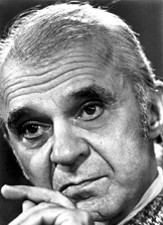
\includegraphics[width=1\linewidth]{Images/discrete_time_systems_10}
\caption{}
\label{fig:discrete_time_systems_10}
\end{figure}
		\end{column}
	\end{columns}


\end{frame}
\begin{frame}
	\frametitle{Example: Leontief model of a planned economy}
	Leontief divided the economy in sectors who buy from eachother.
	To produce one unit of industry 0.40 units of agriculture are required
	TABEL INPORTEREN
\end{frame}
\begin{frame}
	\frametitle{Example: Leontief model of a planned economy}
		     :production of sector i in month k
		     :the demand to goods from sector i in the next month
		     Note: in planned economy demand can be steered, economists can decide how many rations they give.
		     The model
		     $ x[k-1] = A x[k] + I u[k]\\
		     y[k] = I x[k]$
		     
		     It is anti-causal: a subdivision of non-causal, for which only future values have to be known to know the current value
		     \hyperlink{http://www.unc.edu/~marzuola/Math547_S13/Math547_S13_Projects/M_Kim_Section001_Leontief_IO_Model.pdf}{More info}
		     
\end{frame}

\section{Z-transform}
\begin{frame}{Z-transform}
	\begin{definition}
		\begin{itemize}
			\item Discrete equivalent to the Laplace-transform
			\item Converts time dependent descriptions of systems to the time-independent Z-domain.
			\item Simplifies many calculations:
			\begin{itemize}
				\item 	Convolution theorem → convolution becomes multiplication
				\item Linear difference equations become simple algebraic expressions
				\item \dots
			\end{itemize}
		\end{itemize}
	
		
	\end{definition}
		\begin{figure}
			\centering
			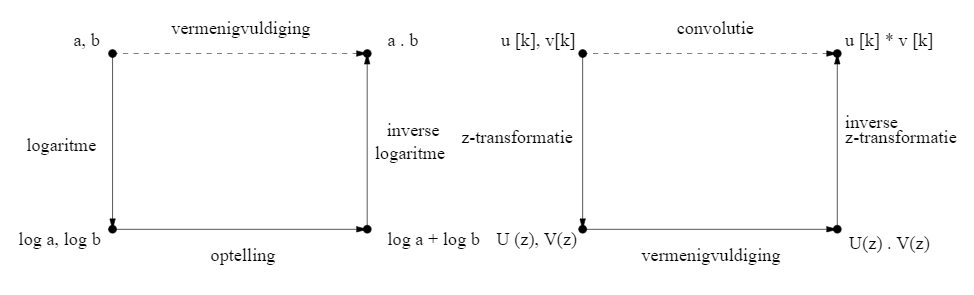
\includegraphics[width=0.7\linewidth]{Images/discrete_time_systems_21}
			\caption{}
			\label{fig:discrete_time_systems_21}
		\end{figure}
		
\end{frame}
\begin{frame}
	\frametitle{Z-transform}
	\begin{block}{2 forms}
			\begin{itemize}
				
				\item Bilateral:
				Requires knowledge of h for all values of k, including negative values
				Can be used for non-causal systems $X(z) = \sum\limits_{k=-\infty}^{\infty} x[k]z^{-k}$
				\item 	Unilateral:
				Only requires knowledge of h for positive values of k
				Can only be used for causal systems without loss of information $X(z) = \sum\limits_{k=0}^{\infty} x[k]z^{-k}$
			\end{itemize}
	\end{block}


\end{frame}
\begin{frame}
	\frametitle{Z-transform}
		\begin{example}
			\begin{center}
				
				$x[k] = \begin{Bmatrix}
				1 & - 1 & 0 & 2 & 4\\
				&     &   & \uparrow & \\
				\end{Bmatrix}$
			\end{center}
			\begin{center}
				$X(z) = \sum\limits_{k=-3}^{1}x[k]z^{-k} = z^3 -z^2 +2 + 4z^{-1}$
			\end{center}
		\end{example}	
\end{frame}
\begin{frame}
	\frametitle{Properties Unilateral Z-transform}
	\small
		\begin{tabular}{|c|c|c|}
			\hline  Propery & Time Domain & Z-domain  \\ 
			\hline  Linearity & $af_1[n]+bf_2[n] + \dots  $& $aF_1(Z)+bF_2(Z)+\dots$ \\ 
			\hline  Right Shift(m$>$0)& $f[k-m]$  &$z^{-m}F(Z)$  \\ 
			\hline  Left Shif (m$>$0)& $f[k+m] $  & $ z^m\bigg(F(z)-\sum\limits_{i=0}^{m-1}f[i]z^{-i} \bigg)$ \\ 
			\hline  Convolution & $f[k]\ast g[k] $  & $F(z)G(z) $ \\ 
			\hline  Multiplication by $a^{k}$ & $a^{k}f[k]$  & $F(a^{-1}z)$  \\ 
			\hline  Summation in time& $\sum\limits_{i=0}^{k}f[i]$  & $\frac{z}{z-1}F(Z) $\\ 
			\hline  Differentation in z& $k^mf[k]$ & $\big(-z \frac{d}{d}\big)^{m} F(z)$ \\ 
			\hline  Periodic Sequence & $f[k] = f[k+N]$  & $F(z) = \frac{z^N}{z^{N-1}}\sum\limits_{k=0}^{N-1}f[k]z^{-1}  \\ 
			\hline  Initial Value& f[0] & \lim_{\mid z \mid \to \infty} F(z) $  \\ 
			\hline  Final value & $f[\infty] $ & $\lim_{z \to 1} (z-1)F(z) $ \\ 
			\hline 
		\end{tabular} 
\end{frame}
\begin{frame}
	\frametitle{List of common Z-transform pairs}
	\begin{figure}
\centering
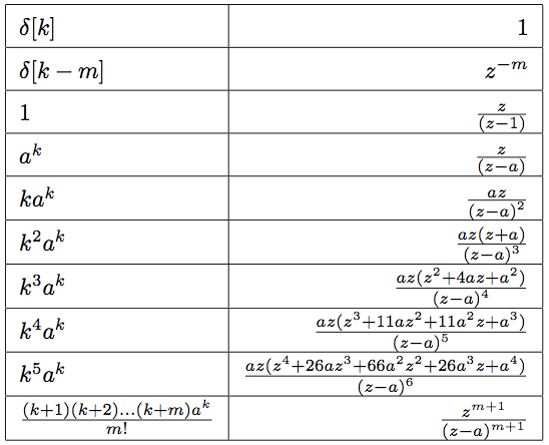
\includegraphics[height=0.8\textheight]{Images/discrete_time_systems_22}

\label{fig:discrete_time_systems_22}
\end{figure}

	
\end{frame}
\begin{frame}
	\frametitle{List of common Z-transform pairs}
	\begin{figure}
\centering
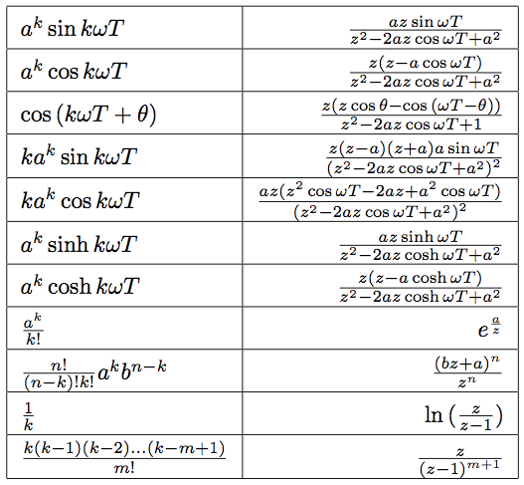
\includegraphics[height=0.8\textheight]{Images/discrete_time_systems_23}
\caption{}
\label{fig:discrete_time_systems_23}
\end{figure}

\end{frame}
\begin{frame}
	\frametitle{Region of convergence}
	\begin{alertblock}{Z-transform not unique}
		Two different signals could have the same Z-transfor over a different region of convergence.
	\end{alertblock}
	\begin{definition}
		The region of convergence is the set of complex numbers z for which:
		\vspace{-2em}
		\begin{center}
			$\sum\limits_{k=-\infty}^{\infty} \mid x[k]z^{-k} \mid < \infty$
		\end{center}
		
	\end{definition}
	
	
\end{frame}
\begin{frame}
		\begin{itemize}
			\item We will look at convergence separately for positive and negative k, splitting the convergence criterion in 2:
			\begin{center}
				$k<0: \mid x[k] \mid \leq M_{-}R_{-}^{k}$\\
				$k\geq 0: \mid x[k] \mid \leq M_{+}R_{+}^{k} $
			\end{center}
			\item Using $z = r e^{j\theta}$ with R+ as small as possible and R- as large as possible we get:
			\begin{center}
				\begin{align}
				\sum\limits_{k=-\infty}^{\infty} \mid x[k]z^{-k} \mid &= \sum\limits_{k=-\infty}^{\infty} \mid x[k] \mid r^{-k} \\
				&= \sum\limits_{k=1}^{\infty} \mid x[-k] \mid r^{k} + \sum\limits_{k=0}^{\infty} \mid x[k] \mid r^{-k} 
				&\leq M_{-} \sum\limits_{k=1}^{\infty} (R_{-}^{-1}r)^{k} + M_{+} \sum\limits_{k= 0}^{\infty}(R_{+}r^{-1})^{k}
				\end{align}
			\end{center}
		\end{itemize}
\end{frame}
\begin{frame}
\frametitle{Region of convergence}
The sums are finite if $R_{-}^{-1}r < 1$ and $R_{+}r^{-1} < 1$
Region of convergence: $R_{+} < R_{-}$
R+< R-: Ring
R-< R+: No ROC
Causal system, for negative k:
$x[k] = 0 \Rightarrow R_{-} = + \infty$
cannot contain any poles of the system
ROC of a stable system always contains
the unit circle.
\begin{figure}
\centering
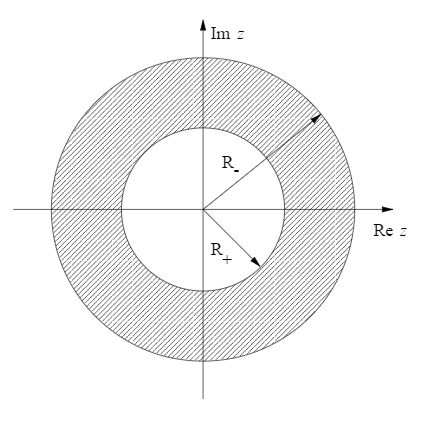
\includegraphics[width=0.4\linewidth]{Images/discrete_time_systems_24}
\caption{}
\label{fig:discrete_time_systems_24}
\end{figure}

\end{frame}
\begin{frame}
	\frametitle{Inverse Z-transform}
	\begin{block}{Inverse Z-transform}
		\begin{enumerate}
			\item Split the function up in partial fractions
			\item Use the table to transform each partial fraction individually to the t-domain
		\end{enumerate}
	\end{block}
	
\end{frame}
\begin{frame}
	\begin{block}{Partial fraction decomposition}
		\begin{enumerate}
			\item Factorizing the denominator
			\item If all poles(zeros of the denominator) have multiplicity 1:
			\vspace{-2 em}
			\begin{center}
				\begin{align}
				F(z) &= \frac{\sum\limits_{i=0}^{n} b_i z^{i}}{a_n(z-p_1)(z-p_2) \dots (z-p_n)}\\
				&= \alpha_0 + \alpha_1 \bigg(\frac{z}{z-p_1}\bigg) + \alpha_2 \bigg(\frac{z}{z-p_2}\bigg) + \dots + \alpha_n \bigg(\frac{z}{z-p_n}\bigg)
				\end{align}
			\end{center}
			\item The coefficients can be calculated by:\\
			\begin{center}
				$\alpha_0 = F(0)$		$\alpha_i = \bigg[\frac{z-p_i}{z} F(z)\bigg]_{z=p_i}$
			\end{center}
			\newcounter{enumTemp}
			\setcounter{enumTemp}{\theenumi}
		\end{enumerate}
	\end{block}
\end{frame}
\begin{frame}
	\frametitle{Inverse Z-transform}
	\begin{enumerate}
		\setcounter{enumi}{\theenumTemp}
		\item If there are poles with multiplicity higher than 1:
		\vspace{-2em}
		\small{
		\begin{center}
			\begin{align}
				F(z) & = \frac{\sum\limits_{i=0}^{n} b_i z^{i}}{a_n(z-p_1)^{n_1}(z-p_2)^{n_2} \dots}\\
				& = \alpha_0 + \alpha_1\bigg(\frac{z}{z-p_1}\bigg) + \alpha_2\bigg(\frac{z}{z-p_1}\bigg)^{2} + \dots + \alpha_{n_1}\bigg(\frac{z}{z-p_1}\bigg)^{n_1} \\
				& + \beta_1 \bigg(\frac{z}{z-p_2}\bigg) + \beta_2 \bigg(\frac{z}{z-p_2}\bigg)^{2} + \dots \beta_{n_2} \bigg(\frac{z}{z-p_2}\bigg)^{n_2}
			\end{align}
		\end{center}
		\item Where the highest coefficient for each pole can be calculated by:
		\begin{center}
			$ \alpha_0 = F(0)$ 		$\alpha_1 = \Bigg[\bigg(\frac{z-p_1}{z}\bigg)^{n_1}F(z)\Bigg]_{z=p_1}$ 	 $\beta_1 = \Bigg[\bigg(\frac{z-p_2}{z}\bigg)^{n_2}F(z)\Bigg]_{z=p_2}$
		\end{center}}
		\newcounter{enumTmp}
		\setcounter{enumTmp}{\theenumi}
	\end{enumerate}
\end{frame}
\begin{frame}
	\frametitle{Inverse Z-transform}
	\begin{enumerate}
		\setcounter{enumi}{\theenumTmp}
		\item Any remaining coefficients can be found by evaluating the equation for a number of values of z.
	\end{enumerate}
\end{frame}
\begin{frame}
	\frametitle{Inverse Z-transform}
	\begin{tabular}{|c|c|}
		\hline $F(z)$ & $f[k]$ \\
		\hline $1$ & $\delta[k]$ \\
		\hline $\frac{z}{z-a}$ & $ a^{k}$ \\
		\hline $\frac{z^{m+1}}{(z-a)^{m+1}}$ & $\frac{(k+1)(k+2)+ \dots (k+m)a^{k}}{m!}$ \\ 
		\hline 
	\end{tabular} 
\end{frame}
\begin{frame}
	\frametitle{Inverse Z-transform}
	\begin{example}
		\begin{center}
			$F(z) = \frac{z^3 + 2 z^2 + z +1}{z^3-z^2-8z +12}$
		\end{center}
		\vspace{-1.5 em}
		\begin{itemize}
			\item The denominator has a zero in 2 (m=2) and -3
			\item Partial fraction decomposition:
			\begin{center}
				$\alpha_0 +\alpha_1 \bigg(\frac{z}{z-2}\bigg)+ \alpha_2 \bigg(\frac{z}{z-2}\bigg)^{2} + \beta_1 \bigg(\frac{z}{z+3}\bigg)$
			\end{center}
			
			\item \begin{center}
				$\alpha_0 = F(0) = \frac{1}{12} $ \\
				$\alpha_2 =\Bigg[\frac{F(z)(z-2)^{2}}{z^2}\Bigg]_{z=2} = \Bigg[\frac{z^3+2z+z+1}{z^2(z+3)}\Bigg]_{z=2} = \frac{19}{20}$\\
				$\beta_1 =\Bigg[\frac{F(z)(z+3)}{z}\Bigg]_{z=-3} = \Bigg[\frac{z^3+2z+z+1}{z(z-2)^2}\Bigg]_{z=-3} = \frac{11}{75}$ 
			\end{center}
		
		\end{itemize}
	\end{example}
\end{frame}
\begin{frame}
	\begin{example}
		\begin{itemize}
				\item By evaluating the function for z=1:\\
				$\frac{5}{4} = \alpha_0 - \alpha_1 + \alpha_2 + \beta/4$\\
				$\alpha_1 = -9/50$
				\item Result : $F(z) = \frac{1}{12} - \frac{9}{50} \frac{z}{z-2} + \frac{19}{20} \frac{z^2}{(z-2)^2} + \frac{11}{75} \frac{Z}{z+3}$
				\item Inverse Z-transform: $f[k] = \gamma[k]/12 + 2^k k \frac{19}{20}
				+ 2^k \frac{77}{100} + (-3)^k \frac{11}{75}$
		\end{itemize}
	\end{example}
\end{frame}
\begin{frame}
	\frametitle{Inverse Z-transform}
	Another technique for calculating the inverse Z-transform is direct division.\\
	The numerator of the transfer function is divided by the denominator via long division.
	\begin{figure}
		\centering
		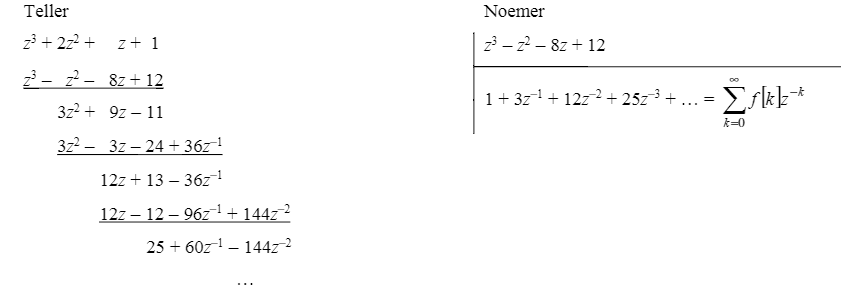
\includegraphics[width=0.9\linewidth]{Images/discrete_time_systems_25}
		\label{fig:discrete_time_systems_25}
	\end{figure}
	
\end{frame}
\begin{frame}
	\frametitle{Solving difference equations with the Z-transform}
	A system is described by a difference equation of the following form:
	\begin{center}
		$\sum\limits_{i=0}^n a_iy[k+i] = \sum\limits_{i=0}^n b_iu[k+i]$
	\end{center}
	After the Z-transform:
	\begin{center}
		$a_0 Y(z) + \sum\limits_{i=1}^{n} a_i z_i \Bigg[Y(z)-\sum\limits_{j=0}^{i-1}y[j]z^{-j}\Bigg] = b_0U(z)+\sum\limits_{i=1}^{n} b_i z_i \Bigg[U(z)-\sum\limits_{j=0}^{i-1}u[j]z^{-j}\Bigg]$
	\end{center}

\end{frame}
\begin{frame}
		\frametitle{Solving difference equations with the Z-transform}
		Rearranged:
		\begin{center}
			$Y(z) = \frac{\sum\limits_{i=1}^{n} b_i z_i}{\sum\limits_{i=1}^{n} a_i z_i} U(z) - \frac{\sum\limits_{i=1}^{n} b_i z_i \Bigg[\sum\limits_{j=0}^{i-1}u[j]z^{-j}\Bigg]-\sum\limits_{i=1}^{n} a_i z_i \Bigg[\sum\limits_{j=0}^{i-1}y[j]z^{-j}\Bigg]}{\sum\limits_{i=1}^{n} a_i z_i}$
		\end{center}
\end{frame}
\begin{frame}
	\frametitle{Solving difference equations with the Z-transform}
	We’ll apply the following transformation of the double summations:\\
	$ \sum\limits_{i=1}^{n} b_i z^i \sum\limits_{j=0}^{i-1}u[j]z^{-j} = \sum\limits_{s=1}^{n}\sum\limits_{j=0}^{n-s}b_{s+j}u[j]	z^{s}$
	\begin{figure}
	\centering
	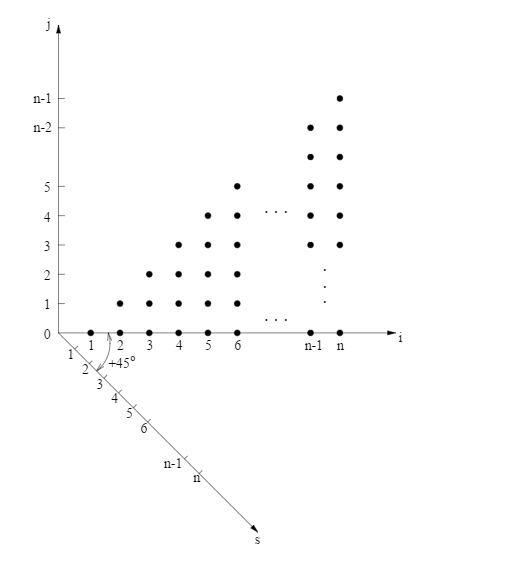
\includegraphics[height = 0.5\textheight]{Images/discrete_time_systems_26}
	\label{fig:discrete_time_systems_26}
	\end{figure}

\end{frame}
\begin{frame}
	\frametitle{Solving difference equations with the Z-transform}
	The final simplified result is:
		$Y(z) = \frac{\sum\limits_{i=1}^{n} b_i z_i}{\sum\limits_{i=1}^{n} a_i z_i} U(z) + \frac{\sum\limits_{s=1}^{n}\Bigg(\sum\limits_{j=0}^{n-s}a_{s+j}y[j]-\sum\limits_{j=0}^{n-s}b_{s+j}u[j]\Bigg)	z^{s}}{\sum\limits_{i=1}^{n} a_i z_}$\\
		With this result it is easy to find the resulting output from a given input or vice-versa given a difference equation.
		Right-hand fraction = output resulting from starting conditions: will vanish with time = transient behavior
		Left-hand fraction = output resulting from input: will remain = steady state response. \\
		$ H(z) = \frac{\sum\limits_{i=1}^{n} b_i z_i}{\sum\limits_{i=1}^{n} a_i z_i}$ is the “transfer function” of the system. This is the z transform of h[k](the impulsresponse)
		
\end{frame}
\begin{frame}
	The transfer function can be derived directly from the state space model of a system:\\
	\begin{center}
		$x[k+1] = Ax[k] + Bu[k] $\\
		$y[k] = Cx[k]+Du[k]$
	\end{center}
	The Z-transform gives:
	\begin{center}
		$z(X(z)-x[0]) = AX(z)+BU(z)$\\
		$Y(z) = CX(z)+DU(z)$
	\end{center}
	Rearranged to have X(z) in explicit form:
	\begin{center}
		$X(z) = (zI-A)^{-1}zx[0] + (zI-A)^{-1}BU(z) $\\
		$Y(z) = C(zI-A)^{-1}zx[0] + \bigg[C(zI-A)^{-1}B + D\bigg]U(z)$
	\end{center}
	If [0] = 0 and $u[k] = \gamma[k] (U(z)=1)$:\\
	$H(z) = C(zI-A)^{-1}B + D$\\
	$Y(z)=H(z)U(z)$
\end{frame}
\begin{frame}
	\frametitle{Z-Transform}
	\begin{definition}
		A pole $p_i$ of of the is system is a point int the complex z-plane where $H(p_i) = \pm \infty$\\
		$\sum\limits_{i=0}^{n}a_iz^{i} = 0$
	\end{definition}
	\begin{definition}
		A zero $n_i$ is a point where $H(n_i)=0$.
		$\sum\limits_{i=0}^{n}b_iz^{i} = 0$
	\end{definition}
\end{frame}
\begin{frame}
	\frametitle{Link between Eigenvalues and poles}
	Are Eigenvalues of A poles of H(z)?\\
	$H(z) = C(zI-A)^{-1}B + D$ \\
	As z approaches an Eigenvalue of A, $(zI-A)^{-1}$ is no longer defined.\\
	$C(zI-A)^{-1}B$	may still be defined depending on the values of C and B.
	\begin{block}{Rule 1}
			An Eigenvalue of A will sometimes, but not always, be a pole of H(z).
	\end{block}
	\begin{definition}
		If every eigenvalue of A is also a pole of H(z) then a minimal number of internal states has been achieved.
	\end{definition}
	
	
\end{frame}
\begin{frame}
	\frametitle{Link between Eigenvalues and poles}
	Are poles of H(z) Eigenvalues of A?
	$H(z) = C(zI-A)^{-1}B + D$ \\
	B, C and D are matrixes with properly defined values
	If H(z) is undefined then $(zI-A)^{-1}$ must be the cause
	z must be an Eigenvalue of A
	\begin{block}{Rule 2}
		Poles of H(z) are always Eigenvalues of A 
	\end{block}
\end{frame}
\begin{frame}
	\frametitle{Stabiltiy}
	\begin{itemize}
		\item Internal Stability
		\begin{itemize}
			\item All possible internal states return to zero after a finite time in the absence of an input.
			\item 	All eigenvalues of the matrix A are contained within the a circle of radius 1 around zero in the complex plane.
		\end{itemize}
		\item BIBO-Stability (Bounded-Input Bounded-Output)
		\begin{itemize}
			\item Every bounded input results in a bounded output
			\item All poles are contained within the a circle of radius 1 around zero in the complex plane
			\item BIBO-Stability follows from Internal Stability, but the inverse is not necessarily true.
		\end{itemize}
	\end{itemize}
\end{frame}
\begin{frame}
	\begin{figure}
\centering
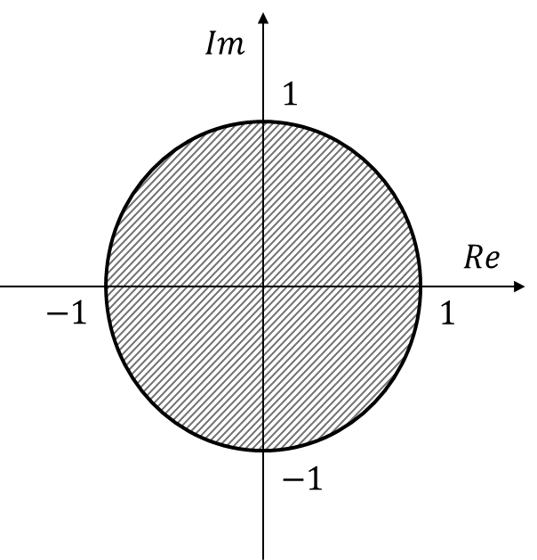
\includegraphics[width=0.7\linewidth]{Images/discrete_time_systems_27}
\caption{}
\label{fig:discrete_time_systems_27}
\end{figure}
\end{frame}
\begin{frame}
	\frametitle{Can unstable systems exist?}
	According to the mathematical models we have discussed unstable systems need an infinite amount of energy.\\
	\textbf{What happens in the real world?}
	\begin{itemize}
		\item The system enters a state in which the current linear model is no longer valid(Non linear behavior) .
		\item Smaller unaccounted effects become more prominent
		\item The system malfunctions and may cause damage to itself or it’s surroundings.
		\item Something else bad happens
	\end{itemize}
\end{frame}
\begin{frame}
	\frametitle{Stability}
	\begin{figure}
	\centering
	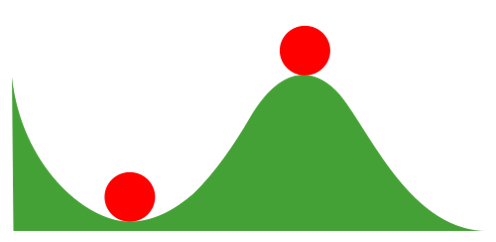
\includegraphics[width=0.7\linewidth]{Images/discrete_time_systems_29}
	\label{fig:discrete_time_systems_29}
	\end{figure}

\end{frame}
\begin{frame}
	\frametitle{Airplane stall}
	\begin{figure}
		\centering
		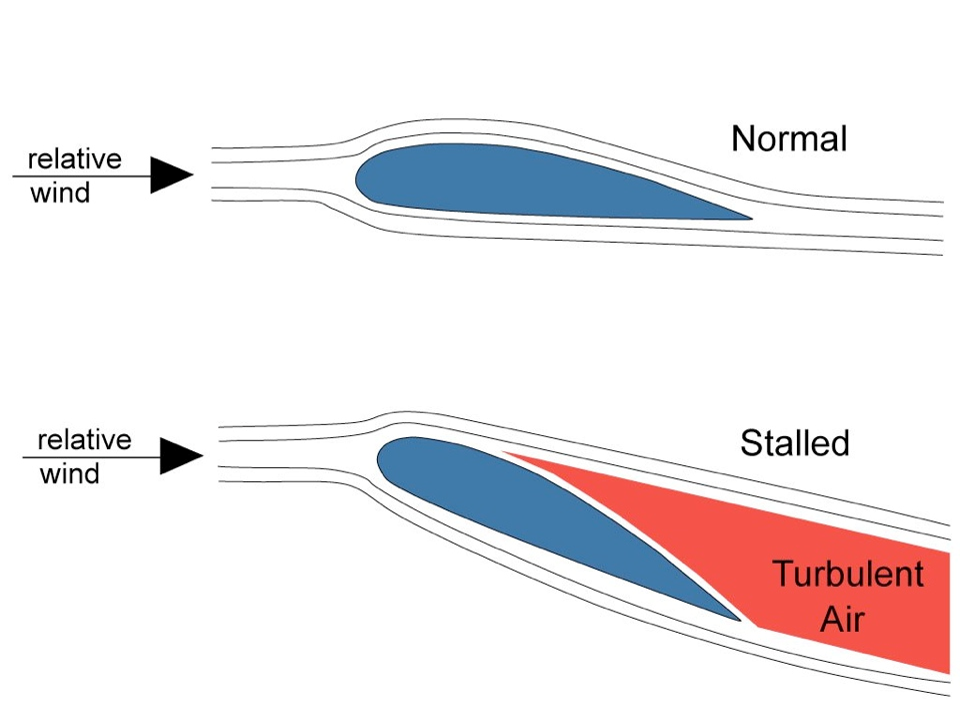
\includegraphics[height=0.7\textheight]{Images/discrete_time_systems_30}
		\label{fig:discrete_time_systems_30}
	\end{figure}
\end{frame}
\begin{frame}
	\begin{itemize}
		\item Airplanes generate lift using the Venturi effect.
		\item Faster moving air has a lower pressure.
		\item Eddy currents may be created due to a too slow airspeed or too sharp ascent.
		\item Turbulent airflow causes a loss of the lift generated by the Venturi effect.
		\item Without the necessary lift an airplane becomes an unstable system.
	\end{itemize}
\end{frame}
\begin{frame}
	\begin{columns}
		\begin{column}{0.6\textwidth}
			Busses and other tall vehicles have a tendency to roll when taking turns too quickly.
			A London bus is loaded with sandbags and must be able to lean at an angle of at least 28˚ while still returning all tires to the ground.
			Modern day car manufacturers have to pass multiple tests for stability while maneuvering
		\end{column}
		\begin{column}
			\begin{figure}
				\centering
				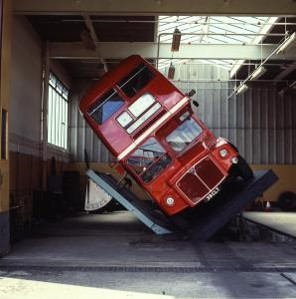
\includegraphics[width=0.8\linewidth]{Images/discrete_time_systems_32}
				\label{fig:discrete_time_systems_32}
			\end{figure}
		\end{column}
	\end{columns}
\end{frame}
\begin{frame}
	
	\frametitle{Steady state behavior via Z-transform}
	Starting from the previous result:\\
	$Y(z) = \frac{\sum\limits_{i=1}^{n} b_i z_i}{\sum\limits_{i=1}^{n} a_i z_i} U(z) + \frac{\sum\limits_{s=1}^{n}\Bigg(\sum\limits_{j=0}^{n-s}a_{s+j}y[j]-\sum\limits_{j=0}^{n-s}b_{s+j}u[j]\Bigg)z^{s}}{\sum\limits_{i=1}^{n}a_i z^i}$\\
	We wish to find the resulting output from the input:\\
	$ u[k] = \cos(k\alpha + \theta)$\\
	To simplify derivation, we use:\\
	$u[k] = e^{j(k\alpha + \theta)}$\\
	With Z-transform:
	$U(z) = \frac{ze^{j\theta}}{z-e^{j\alpha}}$
	
\end{frame}
\begin{frame}
	\frametitle{Steady state behavior via Z-transform}
	Filling in U(z) and splitting into partial fractions:
	
		$Y(z) = \frac{\sum\limits_{i=1}^{n} b_i z_i}{\sum\limits_{i=1}^{n} a_i z_i} \frac{ze^{j\theta}}{z-e^{j\alpha}} + \frac{\sum\limits_{s=1}^{n}\Bigg(\sum\limits_{j=0}^{n-s}a_{s+j}y[j]-\sum\limits_{j=0}^{n-s}b_{s+j}u[j]\Bigg)	z^{s}}{\sum\limits_{i=1}^{n} a_i z_}$\\
		$Y(z) = \frac{cz}{z-e^{j\alpha}} + \frac{d_1z}{z-p_1} + \dots + \frac{d_nz}{z-p_n}+g$\\
	Calculating the coefficient c:\\
	$c= \bigg[Y(z)\frac{z-e^{j\alpha}}{den}\bigg]_{z=e^{j\alpha}} = \bigg[H(z)e^{j\theta}\bigg]_{z=e^{j\alpha} = H(e^{j\alpha})e^{j\theta}$\\
	After the inverse Z-transform:\\
	$
	\begin{align}
			$y[k]&=H(e^{j\alpha})e^{j(k\alpha+\theta)}+d_1p_1^k+\dots+d_np_n^{k}+g\gamma[k]$\\
			$ &= \mid H(e^{j\alpha}) \mid e^{j(k\alpha+\theta+\angle H(e^{j\alpha}))} +d_1p_1^k+\dots+d_np_n^{k}+g\gamma[k]$\\
	\end{align}
	$
\end{frame}
\begin{frame}
	\frametitle{Steady state behavior via Z-transform}
	Because of linearity we can ignore the imaginary component, leading to the result:\\
	$y[k] =  \mid H(e^{j\alpha}) \mid cos(k\alpha+\theta+\angle H(e^{j\alpha})) + Re(d_1p_1^k+\dots+d_np_n^{k}+g\gamma[k])$\\
	\begin{tabular}{|c|c|}
		\hline Input & Output \\ 
		\hline $cos(k\alpha + \theta)$ &  $\mid H(e^{j\alpha}) \mid cos(k\alpha+\theta+\angle H(e^{j\alpha}))$ \\ 
		\hline 
	\end{tabular} 
\end{frame}
\begin{frame}
	\frametitle{Steady state behavior via Z-transform}
	\begin{example}
		\begin{itemize}
			\item $u[k] = cos(3k+\pi) \Rightarrow \alpha = 3 \& \theta = pi$
			\item $H(z) = \frac{z^2+4}{(z^2+6)(z-1)}$
			\item $H(e^3j) = 0.357e^{0.055j}$
			\item The resulting output has been reduced to a third in amplitude and has undergone a small phase shift. \\
			$ y[k] =0.357 \cos(3k+\pi + 0.055)$
			
		\end{itemize}
	\end{example}
\end{frame}
\begin{frame}
	\frametitle{Complex Eigenvalues }
	As with the roots to the characteristic equation in difference equations, complex and/or negative Eigenvalues for A create oscillation.
	The magnitude of the oscillation will grow/decline with          .
	$\lVert\lambda\rVert < 1$: The oscillation will decrease in magnitude: stable
	$\lVert\lambda\rVert > 1$: The oscillation will increase in magnitude:  unstable
	$\lVert\lambda\rVert = 1$: The oscillation will maintain the same magnitude indefinitely:  unstable
	
	The smallest achievable period is 2 times the step time, for negative real eigenvalues.
	
\end{frame}
\begin{frame}
		\frametitle{Complex Eigenvalues }
		\begin{figure}
			\centering
			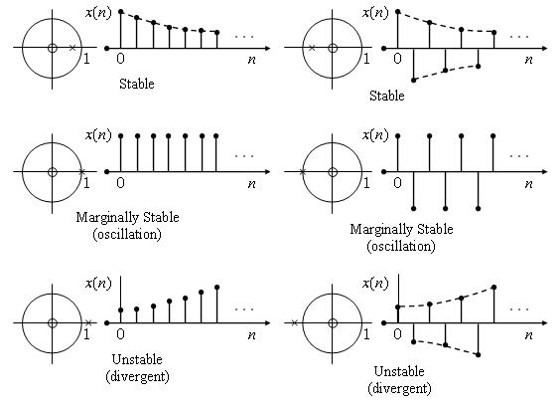
\includegraphics[width=0.7\linewidth]{Images/discrete_time_systems_33}
			\label{fig:discrete_time_systems_33}
		\end{figure}
\end{frame}
\begin{frame}
	\begin{figure}
\centering
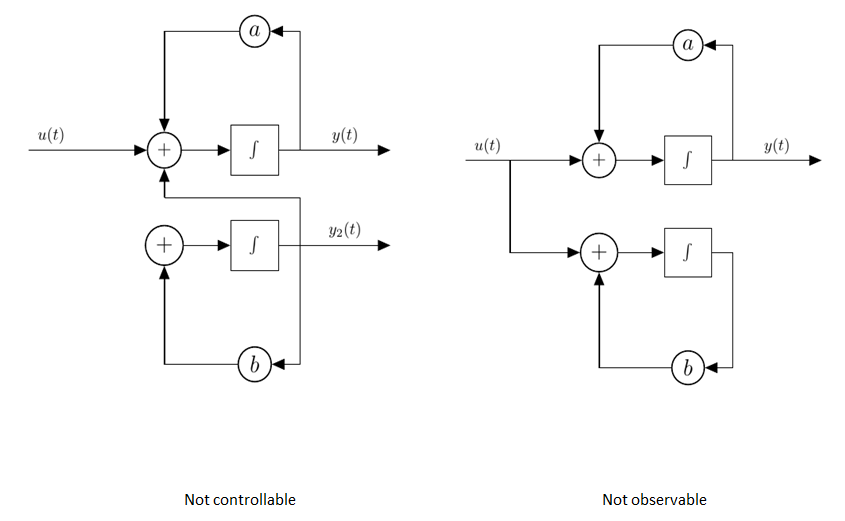
\includegraphics[width=0.7\linewidth]{Images/discrete_time_systems_34}
\caption{}
\label{fig:discrete_time_systems_34}
\end{figure}
\end{frame}
\begin{frame}
	\frametitle{Observability}
	A system is observable if the current state can be determined in finite time by measuring the outputs.\\
	The state space model without inputs gives us:\\
	$x[k+1] = A x[k] $ 				$y[k]=Cx[k]$\\
	Now we can determine a set of vector equations in $x[0]$:\\
	$x[1] = A x[0],x[2]  = A^2x[0],\dots , x[n-1] = A^{n-1} x[0]$\\
	If x[k] has n internal states then n equations are needed:\\
	$y[0] =Cx[0],y[1]=Cx[1]=CAx[0],\dots, y[n-1] = C A^{n-1} x[0]$\\
	$
	\begin{bmatrix}
		C\\
		CA\\
		\vdots\\
		CA^{n-1}\\
	\end{bmatrix}
	x[0]=
	\begin{bmatrix}
		y[0]\\
		y[1]\\
		y[2]\\
		\vdots \\
		y[n-1]\\
	\end{bmatrix}
	$
\end{frame}
\begin{frame}
	\frametitle{Observability}
	A system is controllable if it can be brought to a desired state using the inputs in a finite time.\\
	Again we start from the state space model:\\
	The following equations can be derived:\\
	$x[k+1] = A x[k] +Bu[k]$\\
	$x[1] = Ax[0]+Bu[0]$\\
	$x[2] = A^2 x[0] + ABu[0] + Bu[1]$\\
	$x[3] = A^3 x[0] + A^2Bu[0]+AB u[1] + Bu[2]$\\
	$\vdots$\\
	$x[n] = A^{n}x[0]+A^{n-1}Bu[0] + \dots + Bu[n-1]$
\end{frame}
\begin{frame}
	\frametitle{Controllability}
	This last equation can be rewritten as:
	$x[n] - A^{n}x[0] = \begin{bmatrix}
	B & AB & \dots & A^{n-1}B
	\end{bmatrix}$ $
	\begin{bmatrix}
	u[n-1]\\
	u[n-2]\\
	\vdots\\
	u[1]\\
	u[0]
	\end{bmatrix}
	 $	
	For a given x[0] and a desired x[n] the required inputs can be found by solving this system.
	$\begin{bmatrix}
		B & AB & \dots & A^{n-1}B
	\end{bmatrix}$ is called the controllability matrix of the system.
	A system is said to be controllable if the set of equations can be solved for a given x[0] and any desired x[n].
	This is the case if the controllability matrix has a rank n.
	
\end{frame}
\begin{frame}
	\frametitle{Detectability and Stabilizability}
	Observability and controllability are important terms in control theory.\\
	Detectability and stabilizability are also often used as weaker constraints.\\
	A system is detectable if all unstable states are observable.\\
	A system is stabilizable if all unstable states are controllable.\\
	Detectability and stabilizability are also important terms in control theory.\\
\end{frame}
\begin{frame}
	\frametitle{Overview}
	\begin{figure}
		\centering
		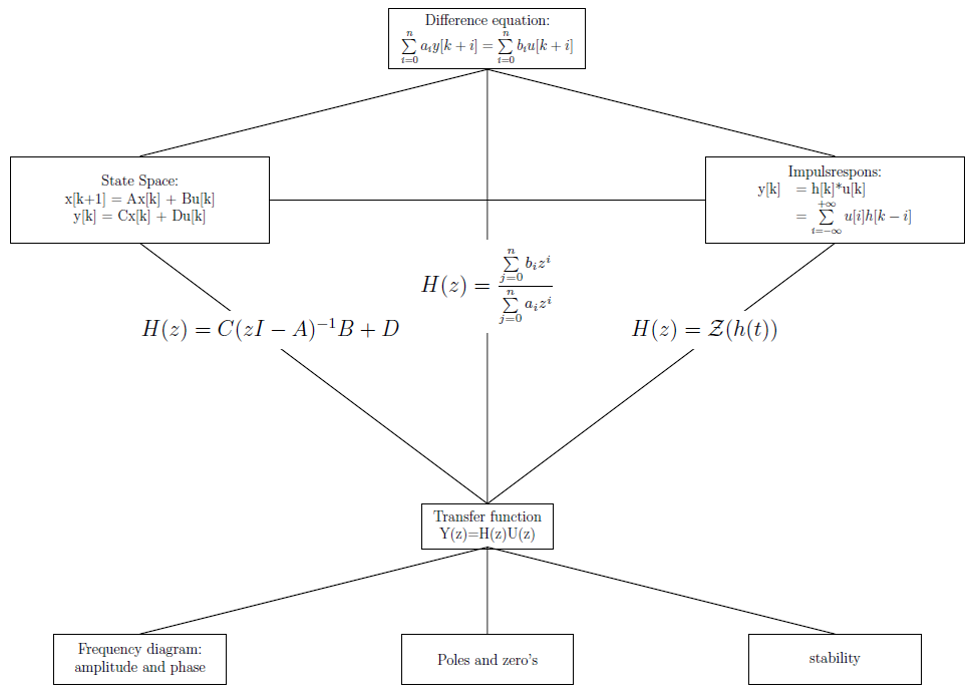
\includegraphics[width=0.7\linewidth]{Images/discrete_time_systems_28}
		\label{fig:discrete_time_systems_28}
	\end{figure}
\end{frame}
